\documentclass[tikz,border=2pt]{standalone}
\usepackage{amsmath,amssymb}
\usepackage{tikz}
\usetikzlibrary{arrows.meta}

\begin{document}
% Marginal pmfs are the row and column totals of the joint table.
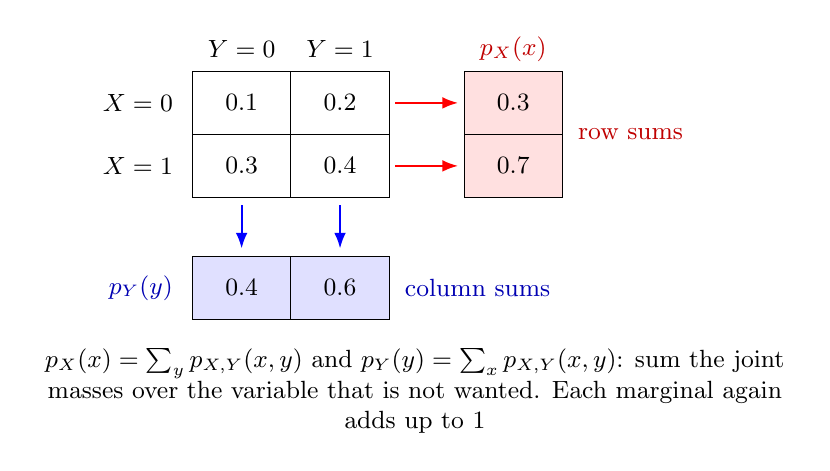
\begin{tikzpicture}[every node/.style={font=\small}, >={Latex[length=2mm]}, cell/.style={draw, minimum width=1.25cm, minimum height=0.8cm}]
	\node[cell] at (0,0) {$0.1$};
	\node[cell] at (1.25,0) {$0.2$};
	\node[cell] at (0,-0.8) {$0.3$};
	\node[cell] at (1.25,-0.8) {$0.4$};
	\node[font=\small] at (0,0.68) {$Y=0$};
	\node[font=\small] at (1.25,0.68) {$Y=1$};
	\node[font=\small, anchor=east] at (-0.75,0) {$X=0$};
	\node[font=\small, anchor=east] at (-0.75,-0.8) {$X=1$};
	\draw[->, red, thick] (1.95,0) -- (2.75,0);
	\draw[->, red, thick] (1.95,-0.8) -- (2.75,-0.8);
	\node[cell, fill=red!12] at (3.45,0) {$0.3$};
	\node[cell, fill=red!12] at (3.45,-0.8) {$0.7$};
	\node[red!75!black, font=\small] at (3.45,0.68) {$p_X(x)$};
	\node[red!75!black, font=\small, anchor=west] at (4.15,-0.4) {row sums};
	\draw[->, blue, thick] (0,-1.3) -- (0,-1.85);
	\draw[->, blue, thick] (1.25,-1.3) -- (1.25,-1.85);
	\node[cell, fill=blue!12] at (0,-2.35) {$0.4$};
	\node[cell, fill=blue!12] at (1.25,-2.35) {$0.6$};
	\node[blue!70!black, font=\small, anchor=east] at (-0.75,-2.35) {$p_Y(y)$};
	\node[blue!70!black, font=\small, anchor=west] at (1.95,-2.35) {column sums};
	\node[anchor=north, align=flush center, text width=9.6cm] at (2.2,-3.0) {$p_X(x)=\sum_yp_{X,Y}(x,y)$ and $p_Y(y)=\sum_xp_{X,Y}(x,y)$: sum the joint masses over the variable that is not wanted. Each marginal again adds up to $1$};
\end{tikzpicture}
\end{document}
